\documentclass{handout}

\SetHandoutTitle{Einfache Wurzeln}
\SetUniversitaet{Karlsruher Institut für Technologie}
\SetDatum{17.06.2019}
\SetSemester{Sommersemester 2019}
\SetDozent{PD Dr.\ Volker Grimm, Dr.\ Ingrid Lenhardt}
\SetReferent{Pavel Zwerschke}
%\SetMatrikelnr{0815}
\SetSeminar{Proseminar SS 2019 Endliche Spiegelungsgruppen}
\SetLiteratur{handout}

\hypersetup{
    pdftitle={Handout \HandoutTitle},
    pdfauthor={\Referent},
    pdfsubject={},
    pdfkeywords={},
    pdfcreator={LaTeX, hyperref, KOMA-Script},
}

\usepackage{../presentation/skript}

\begin{document}

\maketitle
\section{Positive und einfache Wurzeln}
\begin{defi}[\( \Delta_t^+ \) und \( \Delta_t^- \)]
    Sei \( t \in V \) so, dass \( \scalarprod{t}{r} \neq 0 
    \; \forall r \in \Delta \).

    \( \Delta \) lässt sich in zwei Teilmengen 
    \( \Delta_t^+ := 
    \set{r \in \Delta \;\vert \; \scalarprod{t}{r} > 0} \) 
    und \( \Delta_t^- := 
    \set{r \in \Delta \;\vert \; \scalarprod{t}{r} < 0} \) 
    aufteilen. 
\end{defi}

Sei \( r \in \Delta_t^+ \). \( \Rightarrow -r \in \Delta_t^- \), 
da \( \scalarprod{t}{-r} = -\scalarprod{t}{r} \).\\
\( \Rightarrow r \) und \( -r \) sind in 
gegensätzlichen Mengen. 
\( \Rightarrow \abs{\Delta_t^+} = \abs{\Delta_t^-}. \)

\section{Einfache Wurzelsysteme}
\begin{defi}[\( t \)-Basis]
    \( \Pi \subset \Delta_t^+ \) heißt \( t \)-Basis, 
    wenn gilt:
    \begin{itemize}
        \item Jedes \( r \in \Delta_t^+ \) ist 
        eine Linearkombination mit ausschließlich 
        nichtnegativen Koeffizienten.
        \item \( \Pi \) ist minimal.
    \end{itemize}
    Es existiert mindestens eine \( t \)-Basis, 
    da \( \Delta \) endlich ist.
\end{defi}

\begin{defi}[\( t \)-positiv]
    \( x \in V \) heißt \(t\)-positiv, wenn 
    die Linearkombination von \(x\) zur 
    Basis ausschließlich nichtnegativ ist.

    Analog für \( t \)-negativ.
\end{defi}

\begin{satz}
    Seien \( r_i, r_j \in \Pi, i \neq j \) und 
    \( \lambda_i, \lambda_j \in \R_+ \). 
    Der Vektor \( x = \lambda_i r_i - \lambda_j r_j \) 
    ist weder \( t \)-positiv noch \( t \)-negativ.
\end{satz}

\begin{satz}
    Seien \( r_i, r_j \in \Pi, i \neq j \), es 
    sei \( S_i \) die Spiegelung an \( r_i \). 

    Dann ist \( S_i r_i \in \Delta_t^+ \) und 
    \( \scalarprod{r_i}{r_j} \leq 0 \).
\end{satz}

\begin{satz}
    Seien \( x_1, \ldots, x_m \in V \) alle auf derselben 
    Seite einer Hyperebene \( \mathscr{P} \). \\
    Falls \( \scalarprod{x_i}{x_j} \leq 0 \) immer wenn 
    \( i \neq j \), dann ist \( \set{x_1, \ldots, x_m} \) 
    linear unabhängig.
\end{satz} 

\begin{satz}
    Sei \( \Pi \) eine \(t\)-Basis von \( \Delta \). Dann ist 
    \( \Pi \) eine Basis für \( V \).
\end{satz}

\begin{satz}
    Es gibt nur eine \( t \)-Basis von \( \Delta \).
\end{satz}
\newpage
\begin{bsp}[\( \mathscr{G} = \mathscr{H}_2^4 \)]\leavevmode \\
    \begin{minipage}[c]{0.2\textwidth}
        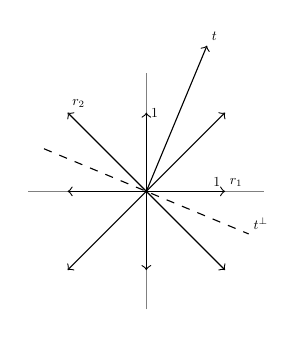
\begin{tikzpicture}
            \draw[thin, gray] (-1.5,0) -- (1.5,0);
            \draw[thin, gray] (0,-1.5) -- (0,1.5);
            \draw[->] (0,0) -- (0,1) node[right, scale=0.5] {\( 1 \)};
            \draw[->] (0,0) -- (0,-1);
            \draw[->] (0,0) -- (-1,0);
            \draw[->] (0,0) -- (1,0) node[above left, scale=0.5] {\( 1 \)};
            \draw (1,0) node[above right, scale=0.5] {\( r_1 \)};
            \draw[->] (0,0) -- (-1, 1);
            \draw (-1, 1) node[above right, scale=0.5] {\( r_2 \)};        
            \draw[->] (0,0) -- (-1,-1);
            \draw[->] (0,0) -- (1,1);
            \draw[->] (0,0) -- (1,-1);
            \draw[->] (0,0) -- (0.77, 1.85) node[above right, scale=0.5] {\( t \)};
            \draw[dashed] (-1.3,-0.77 / 1.85 * -1.3) -- (1.3, -0.77 / 1.85 * 1.3) 
            node[above right, scale=0.5] {\( t^\bot \)};
        \end{tikzpicture}
    \end{minipage}
    \begin{minipage}[c]{0.8\textwidth}
        \[ \Delta = \set{ \pm(1,0), \pm(0,1), (\pm 1, \pm 1) }. \]
        \[ t = 2\left( \cos(\frac{3\pi}{8}), \sin(\frac{3\pi}{8}) \right). \]
        \[ \Rightarrow \Pi = \set{ (1,0), (-1, 1) }. \]
    \end{minipage}
\end{bsp}
\section{Spiegelungsgruppen generieren}
\begin{satz}
    Sei \( S_i \) die Spiegelung an 
    \( r_i \in \Pi = \set{r_1, \ldots, r_n} \).
    Wenn \( r \in \Delta^+ \) und \( r_i \neq r \), 
    dann gilt \( S_i r \in \Delta^+ \).
\end{satz}
\begin{satz}
    Sei \( r \in \Delta^+ \). Es existiert ein \( T \in 
    \mathscr{G}_t := \langle 
    \set{S_i \;\vert\; r_i \in \Pi} \rangle \) so, dass 
    \( Tr \in \Pi \).
\end{satz}

\begin{satz}
    Die einfachen Spiegelungen \( S_1, \ldots, S_n \) 
    erzeugen \( \mathscr{G} \).
\end{satz}

\makeliteratur{}
\end{document}